%
%%%%%%%%%%%%%%%%%%%%%%%%%%%%%%%%%%%%%%%%%%%%%%%%%%%%%%
%                                                    %
%     Modelo para Trabalho de Conclusao de Curso     %
%                                                    %
%                   Template LaTeX                   %
%                                                    %
% Elaboracao  : Grupo PET-Tele                       %
%                                                    %
% Responsaveis:                                      %
%               Marcio Camoleze de Andrade (2008)    %
%               Thiago Muniz de Souza (2008)         %
%                                                    %
% Orientacao  : Prof. Alexandre Santos de la Vega    %
%                                                    %
% Versoes:                                           %
%   - dez/2021 (atualizacao em revisao)              %
%   - set/2017 (primeira revisao estavel)            %
%   - abr/2008 (primeira versao  estavel)            %
%                                                    %
%%%%%%%%%%%%%%%%%%%%%%%%%%%%%%%%%%%%%%%%%%%%%%%%%%%%%%
%

%
\documentclass[12pt,a4paper,oneside]{book}
%
%
%%%%%%%%%%%%%%%%%%%%%%%%%%%%%%%%%%%%%%%%%%%%%%%%%%%%%%
%                Inclusao de pacotes                 %
%%%%%%%%%%%%%%%%%%%%%%%%%%%%%%%%%%%%%%%%%%%%%%%%%%%%%%
%
%
%
%%%%%%%%%%%%%%%%%%%%
%   Pacotes gerais %
%%%%%%%%%%%%%%%%%%%%
%
%
% Padrao brasileiro:
%   a primeira frase eh indentada
%   para todos os paragrafos.
%
\usepackage{indentfirst}
%
%
% Pacotes para lingua portuguesa
%
%%%\usepackage{babel}
%%%\usepackage[brazil]{babel}
\usepackage[brazilian]{babel}
%%%\usepackage[portuguese]{babel}
%%%\babelprovide[import=pt-BR,main]{portuguese}
%
%
%%%\usepackage{ae}
\usepackage{lmodern}
\usepackage[T1]{fontenc}
%
%
% Padrao de codificacao 
% dos caracteres no arquivo '.tex'
%
%%%\usepackage{inputenc}
%\usepackage[ansinew]{inputenc}
\usepackage[utf8]{inputenc}
%
%
% Pacotes matematicos
%
% Package dependency hierarchy 
% in terms of the AMS-LaTeX bundle:
%
% - amsmath (miscellaneous enhancements)
%   - amstext (text embedded in mathematics)
%     - amsgen (*)
%
% - amsbsy (bold symbols)
%   - amsgen (*)
%
% - amsopn (operator name commands)
%   - amsgen (*)
%
% - amssymb (extended symbol collection)
%   - amsfonts (*)
%
% - amsthm (theorem-like environments)
%
% (*) This package has no dependencies.
%
\usepackage{amsmath}
\usepackage{amsfonts}
\usepackage{amssymb}

%
%
% Pacotes graficos
%
%\usepackage{graphics}
\usepackage{graphicx}
\usepackage{subfig}
%\usepackage{subfigure}
\usepackage{epsfig}
%\usepackage{rotating}
%
%
% Pacotes sobre tabelas
%
\usepackage{multirow}
%
%
% Pacote para fazer 'Indice Remissivo'
%
%%%\usepackage{makeidx}
\usepackage{imakeidx}
\makeindex[intoc]
%
%
% Pacotes uteis para revisao do texto
%
% Comentarios de varias linhas
%
\usepackage{comment}
%
%
%%%%%%%%%%%%%%%%%%%%%
% Incluir Códigos   %
%%%%%%%%%%%%%%%%%%%%%
\usepackage{listings}
%
%% Configuracoes do pacote listings
\lstdefinestyle{mystyle}{
language=Python,
basicstyle=\ttm,
% Add keywords here
morekeywords={self, if, True, False, for, except, raise, return, try},
keywordstyle=\ttb\color{deepblue},
% Custom highlighting
emph={set_mode, set_servo_pulsewidth, sleep, OUTPUT, stop, exit},          
% Custom highlighting style
emphstyle=\ttb\color{deepred},    
stringstyle=\color{deepgreen},
% Any extra options here
frame=single,                       
showstringspaces=false,
commentstyle=\color{green}
}
% 
\lstset{
style=mystyle,
breaklines=true
}
%
%
% definicao de comando para Lista de Códigos
%
% Listing -> Código
\renewcommand{\lstlistingname}{Código}
% List of Listings -> Lista de Códigos
\renewcommand{\lstlistlistingname}{Lista de \lstlistingname s}
%
%% PACOTES QUE SERÃO REMOVIDOS APÓS REVISÃO
% Realce de texto
\usepackage{soulutf8}
\usepackage{soul}
% Extensão de letras gregas (Vou tentar Excluir isso)
\usepackage{upgreek}

%%%%%%%%%%%%%%%%% FIM DESSES PACOTES %%%%%%%%%%%%%%

% Marcacao de texto com cor
%
% Explicar...
%
%%%\usepackage{color}
%\usepackage{xcolor}
\usepackage[table,xcdraw]{xcolor}
%
\definecolor{red}  {rgb}{1,0,0}
\definecolor{green}{rgb}{0,1,0}
\definecolor{blue} {rgb}{0,0,1}
\definecolor{deepblue}{rgb}{0,0,0.5}
\definecolor{deepred}{rgb}{0.6,0,0}
\definecolor{deepgreen}{rgb}{0,0.5,0}
\definecolor{green}{rgb}{0,0.8,0}
%
\DeclareFixedFont{\ttb}{T1}{txtt}{bx}{n}{12} % for bold
\DeclareFixedFont{\ttm}{T1}{txtt}{m}{n}{12}  % for normal
%
%
% O pacote 'xurl' 
% faz quebra automatica de linha 
% para um URL muito grande...
%
%%%\usepackage{url}
\usepackage{xurl}
%
\usepackage{hyperref}
%
%
% Explicar e posicionar...
%
%%%\usepackage{memhfixc}
%

%%%%%%%%%%%%%%%%%%%%%%%%%%%%%%%%%%%%%%%%%%%%%%%%%%%%%%
%
%
%%%%%%%%%%%%%%%%%%%%%%%%%%%%%%%%%%%%%%%%%%%%%%%%%%%%%%
%              Formatacao da Pagina                  %
%%%%%%%%%%%%%%%%%%%%%%%%%%%%%%%%%%%%%%%%%%%%%%%%%%%%%%
%
%%%%%%%%%%%%%%%%%%%%%%%%%%%%%%%%%%%%%%%%%%%%%%%%%%%%%%
%              Formatacao da Pagina                  %
%%%%%%%%%%%%%%%%%%%%%%%%%%%%%%%%%%%%%%%%%%%%%%%%%%%%%%

%
% Paper size A4: width=210mm ; height=297mm
%

% horizontal
\setlength{\hoffset}{-1in}

\setlength{\oddsidemargin}{3.0cm} 

\setlength{\textwidth}{160mm}  % (210mm - 30mm - 20mm)

\setlength{\parindent}{1.25cm} % indentacao de cada paragrafo

% vertical
\setlength{\voffset}{-1in}
\addtolength{\voffset}{2.0cm}

\setlength{\topmargin}{0.0cm}

\setlength{\headheight}{5mm}
\setlength{\headsep}{5mm}

\setlength{\textheight}{247mm} % (297mm - 30mm - 20mm)

%%%\setlength{\footskip}{0mm}

%%%%%%%%%%%%%%%%%%%%%%%%%%%%%%%%%%%%%%%%%%%%%%%%%%%%%%
%
%
%%%%%%%%%%%%%%%%%%%%%%%%%%%%%%%%%%%%%%%%%%%%%%%%%%%%%%
%                     Definicoes                     %
%%%%%%%%%%%%%%%%%%%%%%%%%%%%%%%%%%%%%%%%%%%%%%%%%%%%%%
%
% espacamento entre linhas: 
%   \linespread{factor}
%   factor=1.0 (espaço simples)
%   factor=1.3 (espaço 1 1/2)
%   factor=1.6 (espaço duplo)
\linespread{1.3} 
%
\pagestyle{myheadings}
%
\makeindex

%%%%%%%%%%%%%%%%%%%%%%%%%%%%%%%%%%%%%%%%%%%%%%%%%%%%%%


%%%%%%%%%%%%%%%%%%%%%%%%%%%%%%%%%%%%%%%%%%%%%%%%%%%%%%
%             Regras de Divisao Silabica             %
%%%%%%%%%%%%%%%%%%%%%%%%%%%%%%%%%%%%%%%%%%%%%%%%%%%%%%

\hyphenation{tra-ba-lho cur-so En-ge-nhei-ro}

%%%%%%%%%%%%%%%%%%%%%%%%%%%%%%%%%%%%%%%%%%%%%%%%%%%%%%

%
\begin{document}
%

%%%%%%%%%%%%%%%%%%%%%%%%%%%%%%%%%%%%%%%%%%%%%%%%%%%%%%
%                  Capa da Monografia                %
%%%%%%%%%%%%%%%%%%%%%%%%%%%%%%%%%%%%%%%%%%%%%%%%%%%%%%

\begin{titlepage}
  \begin{center}
    \Large{\textsc{Universidade Federal Fluminense} \\
           \textsc{Escola de Engenharia} \\
           \textsc{Curso de Graduação em Engenharia de Telecomunicações} 
          }
    \par\vfill
    \LARGE{Lúcio Folly S. Zebendo\\e\\João Luiz de Amorim P. Neto}
    \par\vfill
    \LARGE{Aplica\c{c}\~{o}es de \textit{Drones} em Redes de Computadores: Utilização da plataforma \textit{Raspberry Pi} como computador de bordo.}
    \par\vfill
    \Large{Niterói -- RJ\\
    2022}
  \end{center}
\end{titlepage}

%%%%%%%%%%%%%%%%%%%%%%%%%%%%%%%%%%%%%%%%%%%%%%%%%%%%%%


%%%%%%%%%%%%%%%%%%%%%%%%%%%%%%%%%%%%%%%%%%%%%%%%%%%%%%
%                   Folha de Rosto                   %
%%%%%%%%%%%%%%%%%%%%%%%%%%%%%%%%%%%%%%%%%%%%%%%%%%%%%%

\begin{center}

Lúcio Folly S. Zebendo\\e\\João Luiz de Amorim P. Neto

\vfill

Aplica\c{c}\~{o}es de \textit{Drones} em Redes de Computadores: Utilização da plataforma \textit{Raspberry Pi} como computador de bordo.

\vspace{3.0cm}

\begin{flushright}
\begin{minipage}{0.55\textwidth}
%
Trabalho de Conclusão de Curso 
apresentado ao Curso de Graduação em Engenharia de Telecomunicações 
da Universidade Federal Fluminense, 
como requisito parcial para obtenção 
do Grau de Engenheiro de Telecomunicações. 
%
\end{minipage}
\end{flushright}

\vspace{3.0cm}

Orientador: Prof. Dr. Alexandre Santos de la Vega

Coorientador - Prof. Dr. Lauro Eduardo Kozovits
\vfill

Niterói -- RJ

2022

\end{center}

\pagebreak

%%%%%%%%%%%%%%%%%%%%%%%%%%%%%%%%%%%%%%%%%%%%%%%%%%%%%%


%%%%%%%%%%%%%%%%%%%%%%%%%%%%%%%%%%%%%%%%%%%%%%%%%%%%%%
%                Numeracao em romano                 %
%%%%%%%%%%%%%%%%%%%%%%%%%%%%%%%%%%%%%%%%%%%%%%%%%%%%%%

\pagenumbering{roman}
\setcounter{page}{2}

%%%%%%%%%%%%%%%%%%%%%%%%%%%%%%%%%%%%%%%%%%%%%%%%%%%%%%


%%%%%%%%%%%%%%%%%%%%%%%%%%%%%%%%%%%%%%%%%%%%%%%%%%%%%%%%
%	            Ficha Catalografica                    %
%%%%%%%%%%%%%%%%%%%%%%%%%%%%%%%%%%%%%%%%%%%%%%%%%%%%%%%%

% 
% Info from LaTeX:
%
% \vspace{\fill} in a paragraph will 
%   add the filling vertical space 
%   below the line in which it eventually appears.
%
%   \vspace*{\fill}: the space is never removed.
%
%
% \vfill ends the paragraph at the spot and 
%   adds the filling vertical space.
%

\vspace*{\fill}

  \begin{figure}[!ht]
    \centering
%
% comando para inserir arquivo de imagem
%
%    \includegraphics[width=0.7\textwidth]{FichaCatalografica.jpg}

%
% box inserida apenas para ilustrar posicao da Ficha Catalografica
%
    \framebox{
      \begin{minipage}{0.7\textwidth}
        \centering
        A figura referente ao arquivo 

        \vspace{1cm}
        
        \textit{FichaCatalografica.jpg} 

        \vspace{1cm}
        
        fornecido pela Biblioteca 

        \vspace{1cm}
        
        deverá aparecer aqui. 

        \vspace{1cm}
        
        \textbf{ATENÇÃO: Na versão impressa, 
                essa página deverá ficar 
                no verso da página anterior.}
      \end{minipage}
    } 
  \end{figure}
%
% box inserida apenas para ilustrar posicao da Ficha Catalografica
%

\vspace*{\fill}

\clearpage

%%%%%%%%%%%%%%%%%%%%%%%%%%%%%%%%%%%%%%%%%%%%%%%%%%%%%%


%%%%%%%%%%%%%%%%%%%%%%%%%%%%%%%%%%%%%%%%%%%%%%%%%%%%%%
%                 Folha de Aprovacao                 %
%%%%%%%%%%%%%%%%%%%%%%%%%%%%%%%%%%%%%%%%%%%%%%%%%%%%%%

\begin{center}

Lúcio Folly S. Zebendo\\e\\João Luiz de Amorim P. Neto

\vspace{1.0cm}

Aplica\c{c}\~{o}es de \textit{Drones} em Redes de Computadores: Utilização da plataforma \textit{Raspberry Pi} como computador de bordo.

\vspace{1.0cm}

\begin{flushright}
\begin{minipage}{0.55\textwidth}
%
Trabalho de Conclusão de Curso 
apresentado ao Curso de Graduação em Engenharia de Telecomunicações 
da Universidade Federal Fluminense, 
como requisito parcial para obtenção 
do Grau de Engenheiro de Telecomunicações. 
%
\end{minipage}
\end{flushright}

\vfill

\begin{flushleft}

Aprovada em DIA de MÊS de ANO.

\end{flushleft}

\vfill

BANCA EXAMINADORA

\vfill

\hrulefill \\
Prof. Dr. Alexandre S. de la Vega - Orientador\\
Universidade Federal Fluminense - UFF

\vfill

\hrulefill \\
Prof. Dr. Lauro Eduardo Kozovits - Co-Orientador\\
Universidade Federal Fluminense - UFF

\vfill

\hrulefill \\
Prof. Alexandre S. de la Vega\\
INSTITUIÇÃO

\vfill

\hrulefill \\
Prof. Lauro Eduardo Kozovits\\
INSTITUIÇÃO

\vfill

Niterói -- RJ

2022

\end{center}

\pagebreak

%%%%%%%%%%%%%%%%%%%%%%%%%%%%%%%%%%%%%%%%%%%%%%%%%%%%%%


%%%%%%%%%%%%%%%%%%%%%%%%%%%%%%%%%%%%%%%%%%%%%%%%%%%%
%            Resumo na lingua vernacula            %
%%%%%%%%%%%%%%%%%%%%%%%%%%%%%%%%%%%%%%%%%%%%%%%%%%%%

\chapter*{Resumo}
%
\addcontentsline{toc}{chapter}{Resumo}
%
\thispagestyle{myheadings}
%
Este trabalho é o fruto de um trabalho conjunto entre vários discentes e docentes da UFF e iniciativa privada, todos com mútuo interesse por VANTs e suas aplicações. O projeto inicial era ideia da Equipe UFFO~\cite{url:equipeuffo} - construir um \textit{drone} para vigilância dos campi da UFF. O hardware a ser utilizado era um quadricóptero equipado com um sistema FPV de transmissão analógica. Posteriormente, houve-se o interesse de equipar um computador de bordo no \textit{drone} em questão, para fazer aplicações no campo da visão computacional com processamento em tempo de voo. Para isso foi utilizado como referência o material da comunidade~\cite{url:ardupilotdoc} sobre computadores de bordo~\cite{url:ardupilot-companioncomputers}.\\
%
Para a escolha do computador de bordo foram levados mais em conta fatores de custo e popularidade, com isso a plataforma \textit{Raspberry Pi}~\cite{url:raspberrypi} foi a selecionada para esse fim.\\
%
A partir da arquitetura proposta, várias aplicações além da visão computacional são possíveis. Como o computador de bordo em questão possui um sistema operacional com propósito geral baseado em \textit{debian}~\cite{url:debian}, além de outras capacidades de Hardware como portas \textit{GPIO} para acoplamento de sensores e atuadores e outros barramentos para conexão de periféricos, as possibilidades para esse hardware são muitas.\\
%
Com isso, a aplicação proposta nesse trabalho será a conexão desse computador de bordo à uma rede IP. Várias capacidades da plataforma \textit{Raspberry Pi} serão exploradas nos experimentos que sucederão, além disso, serão escritos softwares para testar o conceito de \textit{Drones} em Redes de computadores.
%

\bigskip

\hl{ Palavras-chave: Raspberry Pi. Drones. VANT. ROS. Equipe UFFO. Robótica. Ardpilot. Pixhawk}

%%%%%%%%%%%%%%%%%%%%%%%%%%%%%%%%%%%%%%%%%%%%%%%%%%%%%%


%%%%%%%%%%%%%%%%%%%%%%%%%%%%%%%%%%%%%%%%%%%%%%%%%%%%%%
%              Resumo na lingua inglesa              %
%                      Abstract                      %
%%%%%%%%%%%%%%%%%%%%%%%%%%%%%%%%%%%%%%%%%%%%%%%%%%%%%%

\chapter*{Abstract}
%
\addcontentsline{toc}{chapter}{Abstract}
%
\thispagestyle{myheadings}
%
This part is destinated to the abstract of your monograph. 
%
It must be written in the vernacular language and 
in an idiom of great popularization 
(English, French, Spanish, for example). 
%
This part should be done at last, because just after finishing the work 
it will be possible an overall understanding of it. 
%
The abstract should not bring any further information, 
it is just the summary of the relevants aspects of the monograph, 
such as work gender, finality, methodology, results and conclusions. 
%
It must be written impersonally, 
to possess an extension from 150 to 500 words 
typed in simple space and in only one paragraph. 
%
It must be followed by the keywords of your monograph. 

\bigskip

Keywords: Monograph. LaTeX. Hints. 

\newpage

%%%%%%%%%%%%%%%%%%%%%%%%%%%%%%%%%%%%%%%%%%%%%%%%%%%%%%


%%%%%%%%%%%%%%%%%%%%%%%%%%%%%%%%%%%%%%%%%%%%%%%%%%%%%%%%
%	                 Dedicatoria                       %
%%%%%%%%%%%%%%%%%%%%%%%%%%%%%%%%%%%%%%%%%%%%%%%%%%%%%%%%

\begin{flushright}
 \begin{minipage}{0.5\textwidth}
  %
  % espaço do topo até o início da dedicatória 
  \vspace{17.0cm} 
  %
  Espaço reservado para a dedicatória.
  %
 \end{minipage}
\end{flushright}



%%%%%%%%%%%%%%%%%%%%%%%%%%%%%%%%%%%%%%%%%%%%%%%%%%%%%%


%%%%%%%%%%%%%%%%%%%%%%%%%%%%%%%%%%%%%%%%%%%%%%%%%%%%%%%%
%	                 Agradecimentos                    %
%%%%%%%%%%%%%%%%%%%%%%%%%%%%%%%%%%%%%%%%%%%%%%%%%%%%%%%%

\chapter*{Agradecimentos}
\addcontentsline{toc}{chapter}{Agradecimentos}

\thispagestyle{myheadings}

Espaço reservado para os agradecimentos.

Agradecer ao Prof. Alexandre

Agradecer ao Prof. Raul

Agradecer ao Prof. Lauro Eduardo

Agradecer ao Programa PET

Agradecer ao Raphael Miranda e a Equipe UFFO

Agradecer ao Fabio e a Empresa 6DDrones

Agradecer a comunidade Arducopter pelo grande esforço colaborativo em desenvolver as ferramentas utilizadas nesse projeto.

Agradecer a Larissa Lauffer, namorada de João, por todo apoio durante vários momentos difíceis.

Agradecer a minha mãe, padastro e avó pela cobrança e incentivo nos estudos


Os agradecimentos devem ser sucintos e específicos
a cada tipo de ajuda, a cada ideia relevante, 
a cada empréstimo significativo, pois um agradecimento
é, de certa forma, um crédito dado a alguém.


%%%%%%%%%%%%%%%%%%%%%%%%%%%%%%%%%%%%%%%%%%%%%%%%%%%%%%


%%%%%%%%%%%%%%%%%%%%%%%%%%%%%%%%%%%%%%%%%%%%%%%%%%%%%%%%
%                   Lista de Figuras                   %
%%%%%%%%%%%%%%%%%%%%%%%%%%%%%%%%%%%%%%%%%%%%%%%%%%%%%%%%
%
\listoffigures
%
\addcontentsline{toc}{chapter}{Lista de Figuras}
%
\thispagestyle{myheadings}
%
%%%%%%%%%%%%%%%%%%%%%%%%%%%%%%%%%%%%%%%%%%%%%%%%%%%%%%


%%%%%%%%%%%%%%%%%%%%%%%%%%%%%%%%%%%%%%%%%%%%%%%%%%%%%%%%
%                   Lista de Tabelas                   %
%%%%%%%%%%%%%%%%%%%%%%%%%%%%%%%%%%%%%%%%%%%%%%%%%%%%%%%%
%
\listoftables
%
\addcontentsline{toc}{chapter}{Lista de Tabelas}
%
\thispagestyle{myheadings}
%
%%%%%%%%%%%%%%%%%%%%%%%%%%%%%%%%%%%%%%%%%%%%%%%%%%%%%%


%%%%%%%%%%%%%%%%%%%%%%%%%%%%%%%%%%%%%%%%%%%%%%%%%%%%%%%%
%                       Sumario                        %
%%%%%%%%%%%%%%%%%%%%%%%%%%%%%%%%%%%%%%%%%%%%%%%%%%%%%%%%
%
\tableofcontents
%
\thispagestyle{myheadings}

\clearpage

%%%%%%%%%%%%%%%%%%%%%%%%%%%%%%%%%%%%%%%%%%%%%%%%%%%%%%


%%%%%%%%%%%%%%%%%%%%%%%%%%%%%%%%%%%%%%%%%%%%%%%%%%%%%%
%                Numeracao em arabico                %
%%%%%%%%%%%%%%%%%%%%%%%%%%%%%%%%%%%%%%%%%%%%%%%%%%%%%%
%
\pagenumbering{arabic}

%%%%%%%%%%%%%%%%%%%%%%%%%%%%%%%%%%%%%%%%%%%%%%%%%%%%%%


%%%%%%%%%%%%%%%%%%%%%%%%%%%%%%%%%%%%%%%%%%%%%%%%%%%%%%%%
%                        Texto                         %
%%%%%%%%%%%%%%%%%%%%%%%%%%%%%%%%%%%%%%%%%%%%%%%%%%%%%%%%

\chapter{Introdução}
%
% retira numeracao da pagina, conforme as normas de apresentacao.
\thispagestyle{empty} 
%
%
Atrelado à popularização da tecnologia, o barateamento dos \textit{drones} tornou-o capaz de ser usado para além do âmbito militar, ganhando espaço nas industrias cinematográficas, esportivas e do entretenimento, fora para o uso pessoal.\\

Somado à isso, com o barateamento e miniaturização dos componentes eletrônicos nas últimas décadas, surgiram diversas plataformas de 

A difusão de estudos sobre possíveis aplicações é, portanto, uma consequência inevitável. Dessa forma, abre-se um leque de possibilidades para explorar as atividades que um VANT (Veículo Aéreo Não Tripulado) pode executar.\\



\section{Motivações}

O sentimento de interesse e empolgação pela tecnologia dos drones dos autores desse texto foram as forças primordiais para a concepção do trabalho que se segue. Tal interesse nasceu dentro da Universidade Federal Fluminense através da equipe UFFO~\cite{url:equipeuffo}, formada por discentes e docentes da universidade.\\

Com a experiência adquirida na confecção de um drone quadcóptero simples, descobriu-se a possibilidade de acoplar a este um Raspberry Pi~\cite{url:raspberrypi} como computador de bordo da aeronave, expandindo suas capacidades.\\

A partir desta ideia, foram realizados estudos para buscar os métodos e tecnologias mais recentes utilizados nessa configuração de drone. Felizmente, muitas dessas tecnologias utilizadas já estavam disponíveis na documentação Open Source do Ardupilot~\cite{url:ardupilotdoc} para o equipamento utilizado.

\section{Objetivo}

Este trabalho objetiva o projeto e construção de um drone capaz de se comunicar numa rede IP, além de estudar algumas aplicações para esse tipo de equipamento.

\section{Resultados esperados}

\begin{itemize}
\item Criação de um ambiente de simulação para a validação dos experimentos propostos.
\item Um sistema de controle e navegação para o drone via rede IP.
\item Um drone capaz de realizar comunicação numa rede IP.    
\end{itemize}

\section{Trabalhos correlacionados}

 - Artigos de Drones LTE

\section{Organização do documento}
Resumir os seguintes pontos:
\begin{enumerate}
    \item Introducao teorica
    \item Definições
    \item Arquitetura Proposta
    \item Metodologia
\end{enumerate}



%

\chapter{Introdução teórica}
%
% retira numeracao da pagina, conforme as normas de apresentacao.
\thispagestyle{empty} 
%


\section{Definições iniciais}

\subsection{Definição de VANT}
VANT - Veículo Aéreo Não Tripulado é uma aeronave projetada para operar sem a presença de um piloto à bordo. 

\subsection{Tipos de VANTs}

\subsection{Componentes dos VANTs de Asa Rotativa}

\subsection{Controladora PixHawk}

\subsection{UART}

\subsection{Telemetria}

\subsection{Protocolo Mavlink}

\subsection{Computadores de Bordo}

\subsection{ROS - Robot Operative System}

\subsection{Drones DJI}

\section{Arquitetura do sistema proposto}

Explicação dos componentes da arquitetura do sistema proposto.
%
%\begin{figure}[ht]
%    \centering
%    \includegraphics{Images/introducao/planta_inicial.png}
%    \caption{Diagrama em blocos da planta didática em configuração original.}
%    \label{fig:planta_inicial}
%\end{figure}


%%%%%%%%%%%%%%%%%%%%%%%%%%%%%%%%
%%%%%%%% Metodologia %%%%%%%%%%%
%%%%%%%%%%%%%%%%%%%%%%%%%%%%%%%%

\chapter{Metodologia}
\label{chapter:Metodologia}
%
% retira numeracao da pagina, conforme as normas de apresentacao.
\thispagestyle{empty} 
%
\section{Pesquisa}


%
\section{Objetivos do método aplicado}
A metodologia aplicada possui objetivo descritivo e exploratório. Com o sistema devidamente construído, faremos experimentos que comprovam algumas possibilidades de uso para o equipamento.

\section{Abordagem}
adotar-se-á uma análise qualitativa dos resultados obtidos a partir da implementação do novo sistema, em observância aos seguintes questionamentos:
\begin{enumerate}
    \item Com o sistema desenvolvido será possível ao professor, operador do sistema. controlar o experimento remotamente?
    \item Com o sistema desenvolvido a turma da disciplina conseguirá acompanhar o experimento em um ambiente diferente do laboratório?
    \item pergunta avaliativa 3
    \item pergunta avaliativa 4
\end{enumerate}
%
%%%%%%%%%%%%%%%%
%

\section{Descrição do problema}


%%%%%%%%%%%%%%%%%%%%%%%%%%%%%%%%%%%%%%%%%%%%%%%%%%%%%%%
%
\chapter{Detalhamento da solução}
%
% retira numeracao da pagina, conforme as normas de apresentacao.
\thispagestyle{empty} 
%


\section {Série de computadores Raspberry Pi}
%
O Raspberry Pi é uma série de computadores de placa única e tamanho reduzido, que recebem a denominação  SoC (\textit{System on Chip})~\cite{url:soc} à qual são conectados os seguintes dispositivos: monitor, teclado, e mouse. 

Desenvolvido no Reino Unido pela \href{https://www.raspberrypi.org/}{Raspberry Pi Foundation} tendo, como principais objetivos, contribuir para inclusão digital, promoção de ensino básico em ciência da computação e empoderamento social. Uma alternativa de ensino com baixo custo para escolas e estudantes~\cite{url:raspberry_wiki}. A Tabela~\ref{tab:Especificacoes} apresenta as especificações técnicas do modelo Raspberry Pi Revision 2 - Element 14, utilizado pelo grupo PET-Tele. 
%
\begin{table}[!htbp]
    \centering
    \begin{tabular}{ |c|c| } 
        \hline
        Chip & Broadcom BCM2835 SoC Full HD Processador de Aplicações Multimídia\\
        \hline
        CPU & 700 Mhz ARM1176JZ-F Processador de Baixa Potência de aplicações \\
        \hline
        GPU & Dois Núcleos, VideoCore IV, Co-Processador de Multimídia \\ 
        \hline
        Memória & 512MB SDRAM  \\
        \hline
        Ethernet & Onboard 10/100 Ethernet com conector RJ-45 \\
        \hline
        USB 2.0 & Dois Conectores USB 2.0 \\ 
        \hline
        Saída de Vídeo & HDMI e Composição RCA (PAL e NTSC) \\ 
        \hline
        Saída de Áudio & Conector 3.5 mm ou HDMI \\
        \hline
        Armazenamento & SD, MMC, SDIO Card Slot \\
        \hline
        Dimensões & 8.6 cm X 5.4 cm X 1.7 cm \\ 
        \hline
    \end{tabular}
    \caption{Especificações técnicas do modelo Raspberry Pi Revision 2 - Element14.}
    \label{tab:Especificacoes}
\end{table}

\pagebreak

Na Figura~\ref{fig:rasp3b.jpg.0} é mostrado uma fotografia do modelo. 
Dentre os 25 Pinos presentes neste Raspberry, 17 podem ser usados como entradas ou saídas de uso geral, 5 como terminais comuns (GND), 2 como fontes de tensão de valor +5V e 2 como fontes de tensão de valor +3.3V. 

%
A Tabela~\ref{tab:Raspberry Pinout} reúne uma descrição de todos os pinos.
%
\begin{figure}[!htbp]
    \centering
    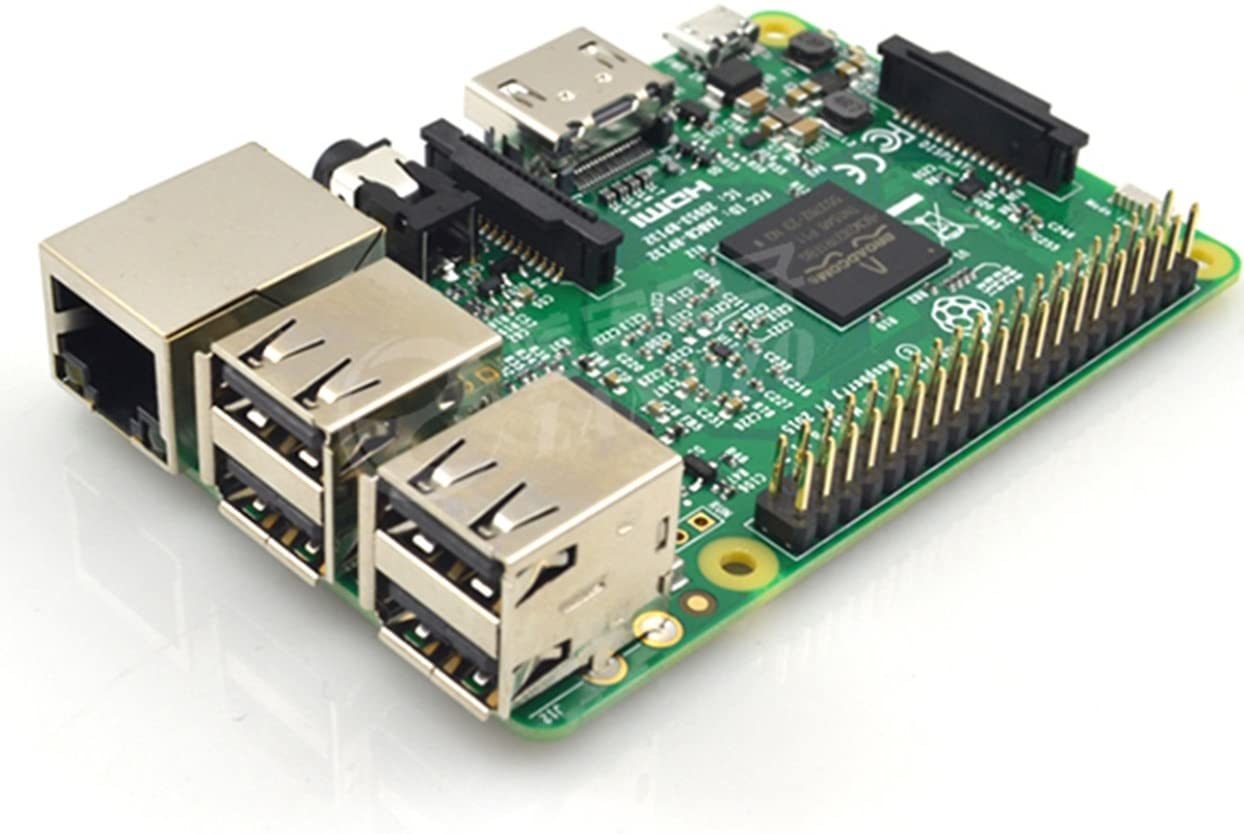
\includegraphics[width=0.7\textwidth]{Images/introducao/rasp3b.jpg}
    \caption{Raspberry Pi Revision 2.0.}
    \label{fig:rasp3b.jpg.0}
\end{figure}
%
\begin{table}[!htbp]
    \centering
    \begin{tabular}{|c|c|c|c|} 
         \hline
         \textbf{N} & \textbf{Descrição} & \textbf{N} & \textbf{Descrição} \\ [0.5ex]
         \hline
         1 & Saída de +3.3V & 14 & Terminal Comum GND\\
         \hline
         2 & Saída de +5V & 15 & GPIO22 \\
         \hline
         3 & GPIO2 | Pull-Up | I2C-SDA & 16 & GPIO23 \\ 
         \hline
         4 & Saída de +5V & 17 & 3V3 \\
         \hline
         5 & GPIO3 | Pull-Up | I2C-SCE & 18 & GPIO24 \\
         \hline
         6 & Terminal Comum GND & 19 & GPIO10 | SPI | MOSI \\ 
         \hline
         7 & GPIO4 & 20 & Terminal Comum GND \\ 
         \hline
         8 & GPIO14 | UART | TXD & 21 & GPIO9 | SPI | MISO\\
         \hline
         9 & Terminal Comum GND & 22 & GPIO25\\
         \hline
         10 & GPIO15 | UART | RXD & 23 & GPIO11 | SPI | CLK\\ 
         \hline
         11 & GPIO17 | UART-RTS & 24 & GPIO8 | SPI | CE0\\
         \hline
         12 & GPIO18 | PWM & 25 & Terminal Comum GND\\ 
         \hline
         13 & GPIO27 & 26 & GPIO7 | SPI | CE1\\ 
         \hline
    \end{tabular}
    \caption{Descrição dos pinos do Raspberry Pi Rev 2.0 - Element 14.}
    \label{tab:Raspberry Pinout}
\end{table}





\chapter{Resultados}
%
% retira numeracao da pagina, conforme as normas de apresentacao.
\thispagestyle{empty} 
%
apresentação de resultados (numéricos e/ou gráficos) 
de cálculos e/ou de simulações, requeridos na especificação do trabalho.

%%%%%%%%%%%%%%%%%%%%%%%%%%%%%%%%%%%%%%%%%%%%%%%%%%%


%%%%%%%%%%%%%%%%%%%%%%%%%%%%%%%%%%%%%%%%%%%%%%%%%%%%%%%%
%                      Conclusão                       %
%%%%%%%%%%%%%%%%%%%%%%%%%%%%%%%%%%%%%%%%%%%%%%%%%%%%%%%%

\chapter{Conclusão}
%
% retira numeracao da pagina, conforme as normas de apresentacao.
\thispagestyle{empty} 
%

\hl{Hipótese testada
Se realizarmos o experimento em outro ambiente com maior capacidade para que todos possam assistir de forma homogênea atenderemos a demanda da turma, teremos um aprendizado mais efetivo e melhoria no tempo dedicado a esse experimento.

Responda as perguntas avaliativas para definir a conclusão}
\begin{enumerate}
    \item Com o sistema desenvolvido será possível ao professor usuário controlar o experimento proposto remotamente?
    \item pergunta avaliativa 2
    \item pergunta avaliativa 3
    \item pergunta avaliativa 4
\end{enumerate}

A presente monografia detalha o processo de pesquisa, projeto e construção de um sistema para atuação em uma planta didática localizada no Laboratório de Drenagem Irrigação e Saneamento~\cite{url:ladisan}.

Utilizando, como base, o documento 
\textbf{Uso de Sensores e Acesso Remoto para a Realização de Aula Prática Sobre Reservatórios de Detenção Aplicados à Drenagem urbana}~\cite{article:tcc_lorraine_maria} 
%
e o artigo 
\textbf{Realização de Aula Prática Remota a Partir de Laboratório Equipado com Modelo Físico Sobre Detenção de Água de Chuva}~\cite{article:lorraine_maria}, 
publicado no COBENGE 2018~\cite{url:cobenge}, 
%
foi desenvolvido um conjunto de melhorias e novos processos que permitem monitoramento e maior e melhor atuação do ``usuário'' (computador remoto localizado na sala de aula) na planta didática operando no Laboratório LaDISan~\cite{url:ladisan}. 
%
O conjunto de melhorias compreende uma câmera com controle remoto, um servomotor acoplado a um registro de admissão de água, uma interface de acesso e um dispositivo Raspberry Pi operando como controlador do servomotor e computador auxiliar para o Arduino. 

Os resultados foram satisfatórios no que tange aos objetivos propostos. 
Foram realizadas duas aulas no ano de 2019, uma no primeiro semestre letivo e outra no segundo semestre.

O sistema ainda não contempla uma solução fechada pronta para comercialização conforme foi citado no Capítulo~\ref{chapter:Metodologia}.
%
Ainda se faz necessário melhorias e correções que podem ser implementadas conforme novas demandas levantadas por alunos da disciplina e o professor Dario Sobrenome Sobrenome.
%
As demandas podem ser implementadas pelos futuros bolsistas do grupo PET-Tele. Complementarmente a este documento existe um relatório técnico com detalhamento das etapas de construção, disponível no \textit{website} do Grupo PET-Tele~\cite{url:projeto_ladisan}

%%%%%%%%%%%%%%%%%%%%%%%%%%%%%%%%%%%%%%%%%%%%%%%%%%%%%%%%
%          Sugestoes para trabalhos futuros            %
%%%%%%%%%%%%%%%%%%%%%%%%%%%%%%%%%%%%%%%%%%%%%%%%%%%%%%%%

\chapter{Sugestões para trabalhos futuros}
%
% retira numeracao da pagina, conforme as normas de apresentacao.
\thispagestyle{empty} 
%
%
Em observância ao caráter amplo e diverso dos conceitos aqui utilizados, diversas vertentes de trabalhos futuros podem ser identificadas. Tais vertentes, assim como os trabalhos individuais em cada uma das vertentes, podem ser listados e resumidos.
%
\begin{enumerate}
    \item Vertente Técnica Funcional
        \begin{enumerate}
            \item Novas interfaces de usuário com mais opções
            \item Desenvolvimento de novas curvas hidrográficas
        \end{enumerate}
    \item Vertente Facilidade de Uso
        \begin{enumerate}
            \item Encapsulamento de hardware em produto final
            \item Simplificação do configuração e uso para usuário final.
        \end{enumerate}
    \item Vertente casos de testes
        \begin{enumerate}
            \item Coleta de indicadores para medir o grau de satisfação da turma com o sistema.
            \item Aumentar o número de testes a fim de identificar falhas.
        \end{enumerate}
\end{enumerate}

Vale ressaltar dentro dessas vertentes a necessidade de realização de mais testes com o sistema em operação como forma de garantir que as funcionalidades propostas estejam com o funcionamento correto.]

Para isso, é de fundamental importância a elaboração de novos casos de uso e simulações teste, bem como a implementação de atualizações otimizadas dos programas desenvolvidos. Uma pesquisa avaliando os parâmetros funcionais qualitativos da interface proposta na Seção~\ref{subsec:nova_interface} pode servir de suporte para as exigências aqui formuladas.

%%%%%%%%%%%%%%%%%%%%%%%%%%%%%%%%%%%%%%%%%%%%%%%%%%%%%%


%%%%%%%%%%%%%%%%%%%%%%%%%%%%%%%%%%%%%%%%%%%%%%%%%%%%%%%%%%%%%%%%%%%
%                  Referencias Bibliograficas                     % 
%%%%%%%%%%%%%%%%%%%%%%%%%%%%%%%%%%%%%%%%%%%%%%%%%%%%%%%%%%%%%%%%%%%

\bibliographystyle{apalike}
%
\bibliography{./MyBibFiles/my_refs}
%
\addcontentsline{toc}{chapter}{\refname}
%
\thispagestyle{myheadings}

%
%%%%%%%%%%%%%%%%%%%%%%%%%%%%%%%%%%%%%%%%%%%%%%%%%%%%

%
%%%%%%%%%%%%%%%%%%%%%%%%%%%%%%%%%%%%%%%%%%%%%%%%
%
%
% Apendices e anexos
%
\appendix
%
%
%%%%%%%%%%%%%%%%%%%%%%%%%%%%%%%%%%%%%%%%%%%%%%%%%%%%%%%%
%
\chapter{Apêndice 1}
%
% retira numeracao da pagina, conforme as normas de apresentacao.
\thispagestyle{empty} 
%
Segue abaixo um guia de instalação completo dos \textit{Softwares} de simulação e suas respectivas dependências para Ubuntu 20.04 LTS.

\section{Intalando o ArduPilot e MavProxy}

\subsection{Clonando o repositório \textit{git} para sua máquina}
\begin{lstlisting}[language=bash]
  $ cd ~
  $ sudo apt install git
  $ git clone https://github.com/ArduPilot/ardupilot.git
\end{lstlisting}

\subsection{Instalando as dependências e recompilando o perfil}
\begin{lstlisting}[language=bash]
  $ cd ardupilot/Tools/environment_install/install-prereqs-ubuntu.sh -y
  $ . ~/.profile
\end{lstlisting}

\subsection{Mudando para a \textit{branch} do ArduCopter}
\begin{lstlisting}[language=bash]
  $ git checkout Copter-4.0.4
  $ git submodule update --init --recursive
\end{lstlisting}

\subsection{Rodando SITL (\textit{Software In The Loop})}
\begin{lstlisting}[language=bash]
  $ cd ~/ardupilot/ArduCopter
  $ sim_vehicle.py -w
\end{lstlisting}

\section{Instalando o Gazebo e o \textit{plugin} do ArduPilot}

\subsection{Atualizando a lista de fontes para \textit{download}}
\begin{lstlisting}[language=bash]
  $ sudo sh -c 'echo "deb http://packages.osrfoundation.org/gazebo/ubuntu-stable `lsb_release -cs` main" > /etc/apt/sources.list.d/gazebo-stable.list'
  $ wget http://packages.osrfoundation.org/gazebo.key -O - | sudo apt-key add -
  $ sudo apt update
\end{lstlisting}

\subsection{Instalando o \textit{plugin} do Gazebo para comunicação com o ArduPilot}
\begin{lstlisting}[language=bash]
  $ cd ~
  $ git clone https://github.com/khancyr/ardupilot_gazebo.git
  $ cd ardupilot_gazebo
  $ mkdir build
  $ cd build
  $ cmake ..
  $ make -j4
  $ sudo make install
  $ echo 'source /usr/share/gazebo/setup.sh' >> ~/.bashrc
  $ echo 'export GAZEBO_MODEL_PATH=~/ardupilot_gazebo/models' >> ~/.bashrc
  $ . ~/.bashrc
\end{lstlisting}

\subsection{Executando a simulação}
\begin{lstlisting}[language=bash]
  No primeiro terminal do linux rode o Gazebo: 
  $ gazebo --verbose ~/ardupilot_gazebo/worlds/iris_arducopter_runway.world
  
  No segundo terminal do linux rode o SITL:
  $ cd ~/ardupilot/ArduCopter/
  $ sim_vehicle.py -v ArduCopter -f gazebo-iris --console
\end{lstlisting}

\section{Instalando o \textit{ROS} e o configurando o \textit{Catkin}}

\subsection{Atualizando a lista de fontes para \textit{download}}
\begin{lstlisting}[language=bash] 
  $ sudo sh -c 'echo "deb http://packages.ros.org/ros/ubuntu $(lsb_release -sc) main" > /etc/apt/sources.list.d/ros-latest.list'
  $ sudo apt install curl
  $ curl -s https://raw.githubusercontent.com/ros/rosdistro/master/ros.asc | sudo apt-key add -
  $ sudo apt update
\end{lstlisting}

\subsection{Instalando o \textit{ROS}}
\begin{lstlisting}[language=bash] 
  $ sudo apt install ros-noetic-desktop-full
\end{lstlisting}

\subsection{Configurando o ambiente}
\begin{lstlisting}[language=bash] 
  $ source /opt/ros/noetic/setup.bash
  $ echo "source /opt/ros/noetic/setup.bash" >> ~/.bashrc
  $ source ~/.bashrc
  $ echo "source /opt/ros/noetic/setup.zsh" >> ~/.zshrc
  $ source ~/.zshrc
\end{lstlisting}

\subsection{Instalando as dependências para os pacotes dos \textit{ROS}}
\begin{lstlisting}[language=bash] 
  $ sudo apt install python3-rosdep python3-rosinstall python3-rosinstall-generator python3-wstool build-essential
  $ sudo apt install python3-rosdep
  $ sudo rosdep init
  $ rosdep update
\end{lstlisting}

\subsection{Configurando o \textit{Catkin}}
\begin{lstlisting}[language=bash] 
  $ sudo apt-get install python3-wstool python3-rosinstall-generator python3-catkin-lint python3-pip python3-catkin-tools
  $ pip3 install osrf-pycommon
  $ mkdir -p ~/catkin_ws/src
  $ cd ~/catkin_ws
  $ catkin init
\end{lstlisting}

\subsection{Instalando as dependências para o \textit{Catkin}}
\begin{lstlisting}[language=bash] 
  $ sudo apt-get install python3-wstool python3-rosinstall-generator python3-catkin-lint python3-pip python3-catkin-tools
  $ pip3 install osrf-pycommon
  $ mkdir -p ~/catkin_ws/src
  $ cd ~/catkin_ws
  $ catkin init
\end{lstlisting}

\subsection{Instalando as \textit{MAVROS} e \textit{MAVLink}}
\begin{lstlisting}[language=bash] 
  $ cd ~/catkin_ws
  $ wstool init ~/catkin_ws/src
  $ rosinstall_generator --upstream mavros | tee /tmp/mavros.rosinstall
  $ rosinstall_generator mavlink | tee -a /tmp/mavros.rosinstall
  $ wstool merge -t src /tmp/mavros.rosinstall
  $ wstool update -t src
  $ rosdep install --from-paths src --ignore-src --rosdistro `echo $ROS_DISTRO' -y
  $ catkin build
\end{lstlisting}

\subsection{Atualizando o arquivo \textit{.bachrc}}
\begin{lstlisting}[language=bash] 
  $ echo "source ~/catkin_ws/devel/setup.bash" >> ~/.bashrc
  $ source ~/.bashrc
\end{lstlisting}

\section{Instalando as dependências geográficas e clonando o repositório de simulação do \textit{Intelligent Quads}}

\subsection{Instalando as dependências geográficas}
\begin{lstlisting}[language=bash] 
  $ sudo ~/catkin_ws/src/mavros/mavros/scripts/install_geographiclib_datasets.sh]
\end{lstlisting}

\subsection{Clonando pacote ROS de simulação do \textit{Intelligent Quads}}
\begin{lstlisting}[language=bash] 
  $ cd ~/catkin_ws/src
  $ git clone https://github.com/Intelligent-Quads/iq_sim.git
  $echo "GAZEBO_MODEL_PATH=${GAZEBO_MODEL_PATH}:$HOME/catkin_ws/src/iq_sim/models" >> ~/.bashrc
  $ cd ~/catkin_ws
  $ catkin build
  $ source ~/.bashrc
\end{lstlisting}

\section{Instalando o \textit{QGround Control}}

\subsection{Alterando permissões e instalando o \textit{QGround Control}}
\begin{lstlisting}[language=bash] 
  $ sudo usermod -a -G dialout $USER
  $ sudo apt-get remove modemmanager
  $ wget https://s3-us-west-2.amazonaws.com/qgroundcontrol/latest/QGroundControl.AppImage
  $ chmod +x ./QGroundControl.AppImage 
  $ ./QGroundControl.AppImage
\end{lstlisting}
%
%%%%%%%%%%%%%%%%%%%%%%%%%%%%%%%%%%%%%%%%%%%%%%%%%%%%%%%%
%
\end{document}
%


%%%%%%%%%%%%%%%%%%%%%%%%%%%%%%%%%%%%%%%%
%     Insercao do Indice Remissivo     %
%%%%%%%%%%%%%%%%%%%%%%%%%%%%%%%%%%%%%%%%
%
% Makeindex Database 
% (baseada nos arquivos: XXX.idx --> xxx.ind --> xxx.ilg)
%
\printindex
%
\addcontentsline{toc}{chapter}{\indexname}
%
\thispagestyle{myheadings}


%%%%%%%%%%%%%%%%%%%%%%%%%%%%%%%%%%%%%%%%%%%%%%%%%%%%%%


%
\end{document}
%

%%%%%%%%%%%%%%%%%
% Fim do modelo %
%%%%%%%%%%%%%%%%%
